\section{Results}\label{results}
After running all seven teacher forcing methods 3 times each, the results for each TF method across the different tests were compared using Kruskal-Wallis, as described in Section~\ref{stat}. 

\subsection{ROUGE Scores}\label{results:rouge}
Before diving into ROUGE scores, it is important to understand the distributions of the ROUGE scores for the purposes of statistical analysis. The data is right (positively) skewed, as visualized in Figures~\ref{fig:r1hists}~and~\ref{fig:r2hists}.

\begin{figure}[h]
  \centering
  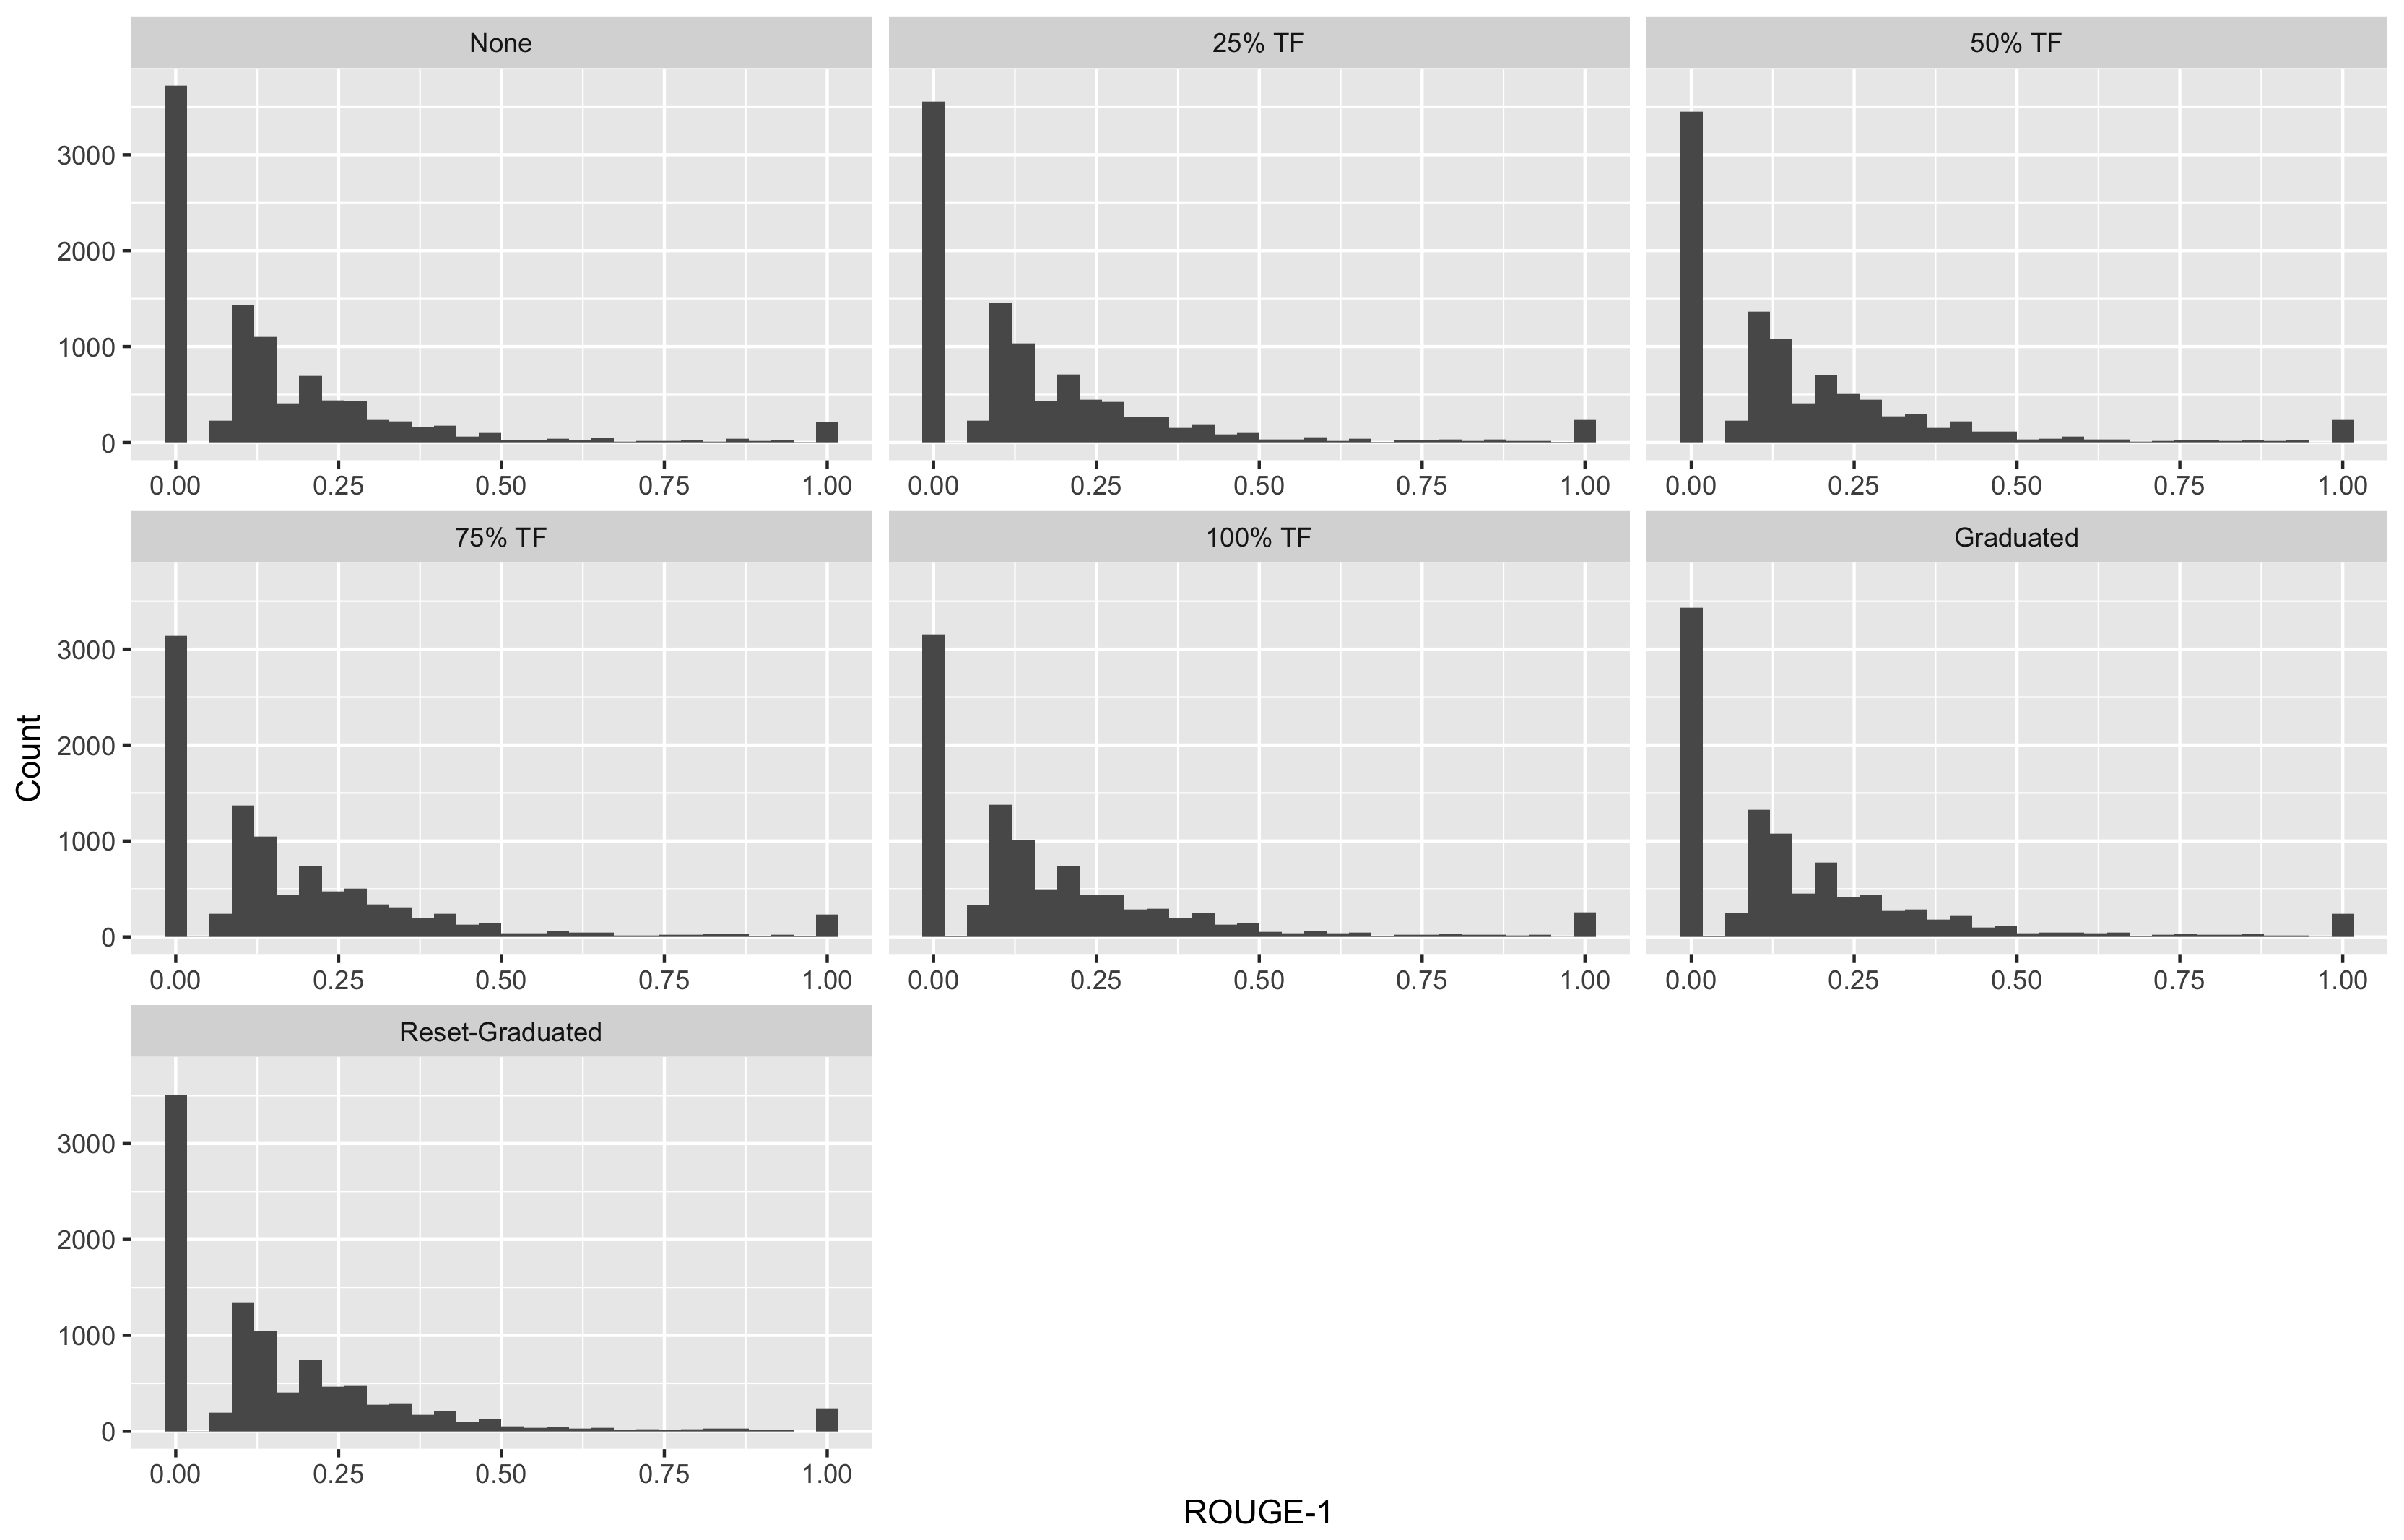
\includegraphics[width=0.8\textwidth]{../plots/test2/r1hists}
  \caption{Histograms of ROUGE-1 scores from all TF methods of Test 2}
  \label{fig:r1hists}
\end{figure}

\begin{figure}[h]
  \centering
  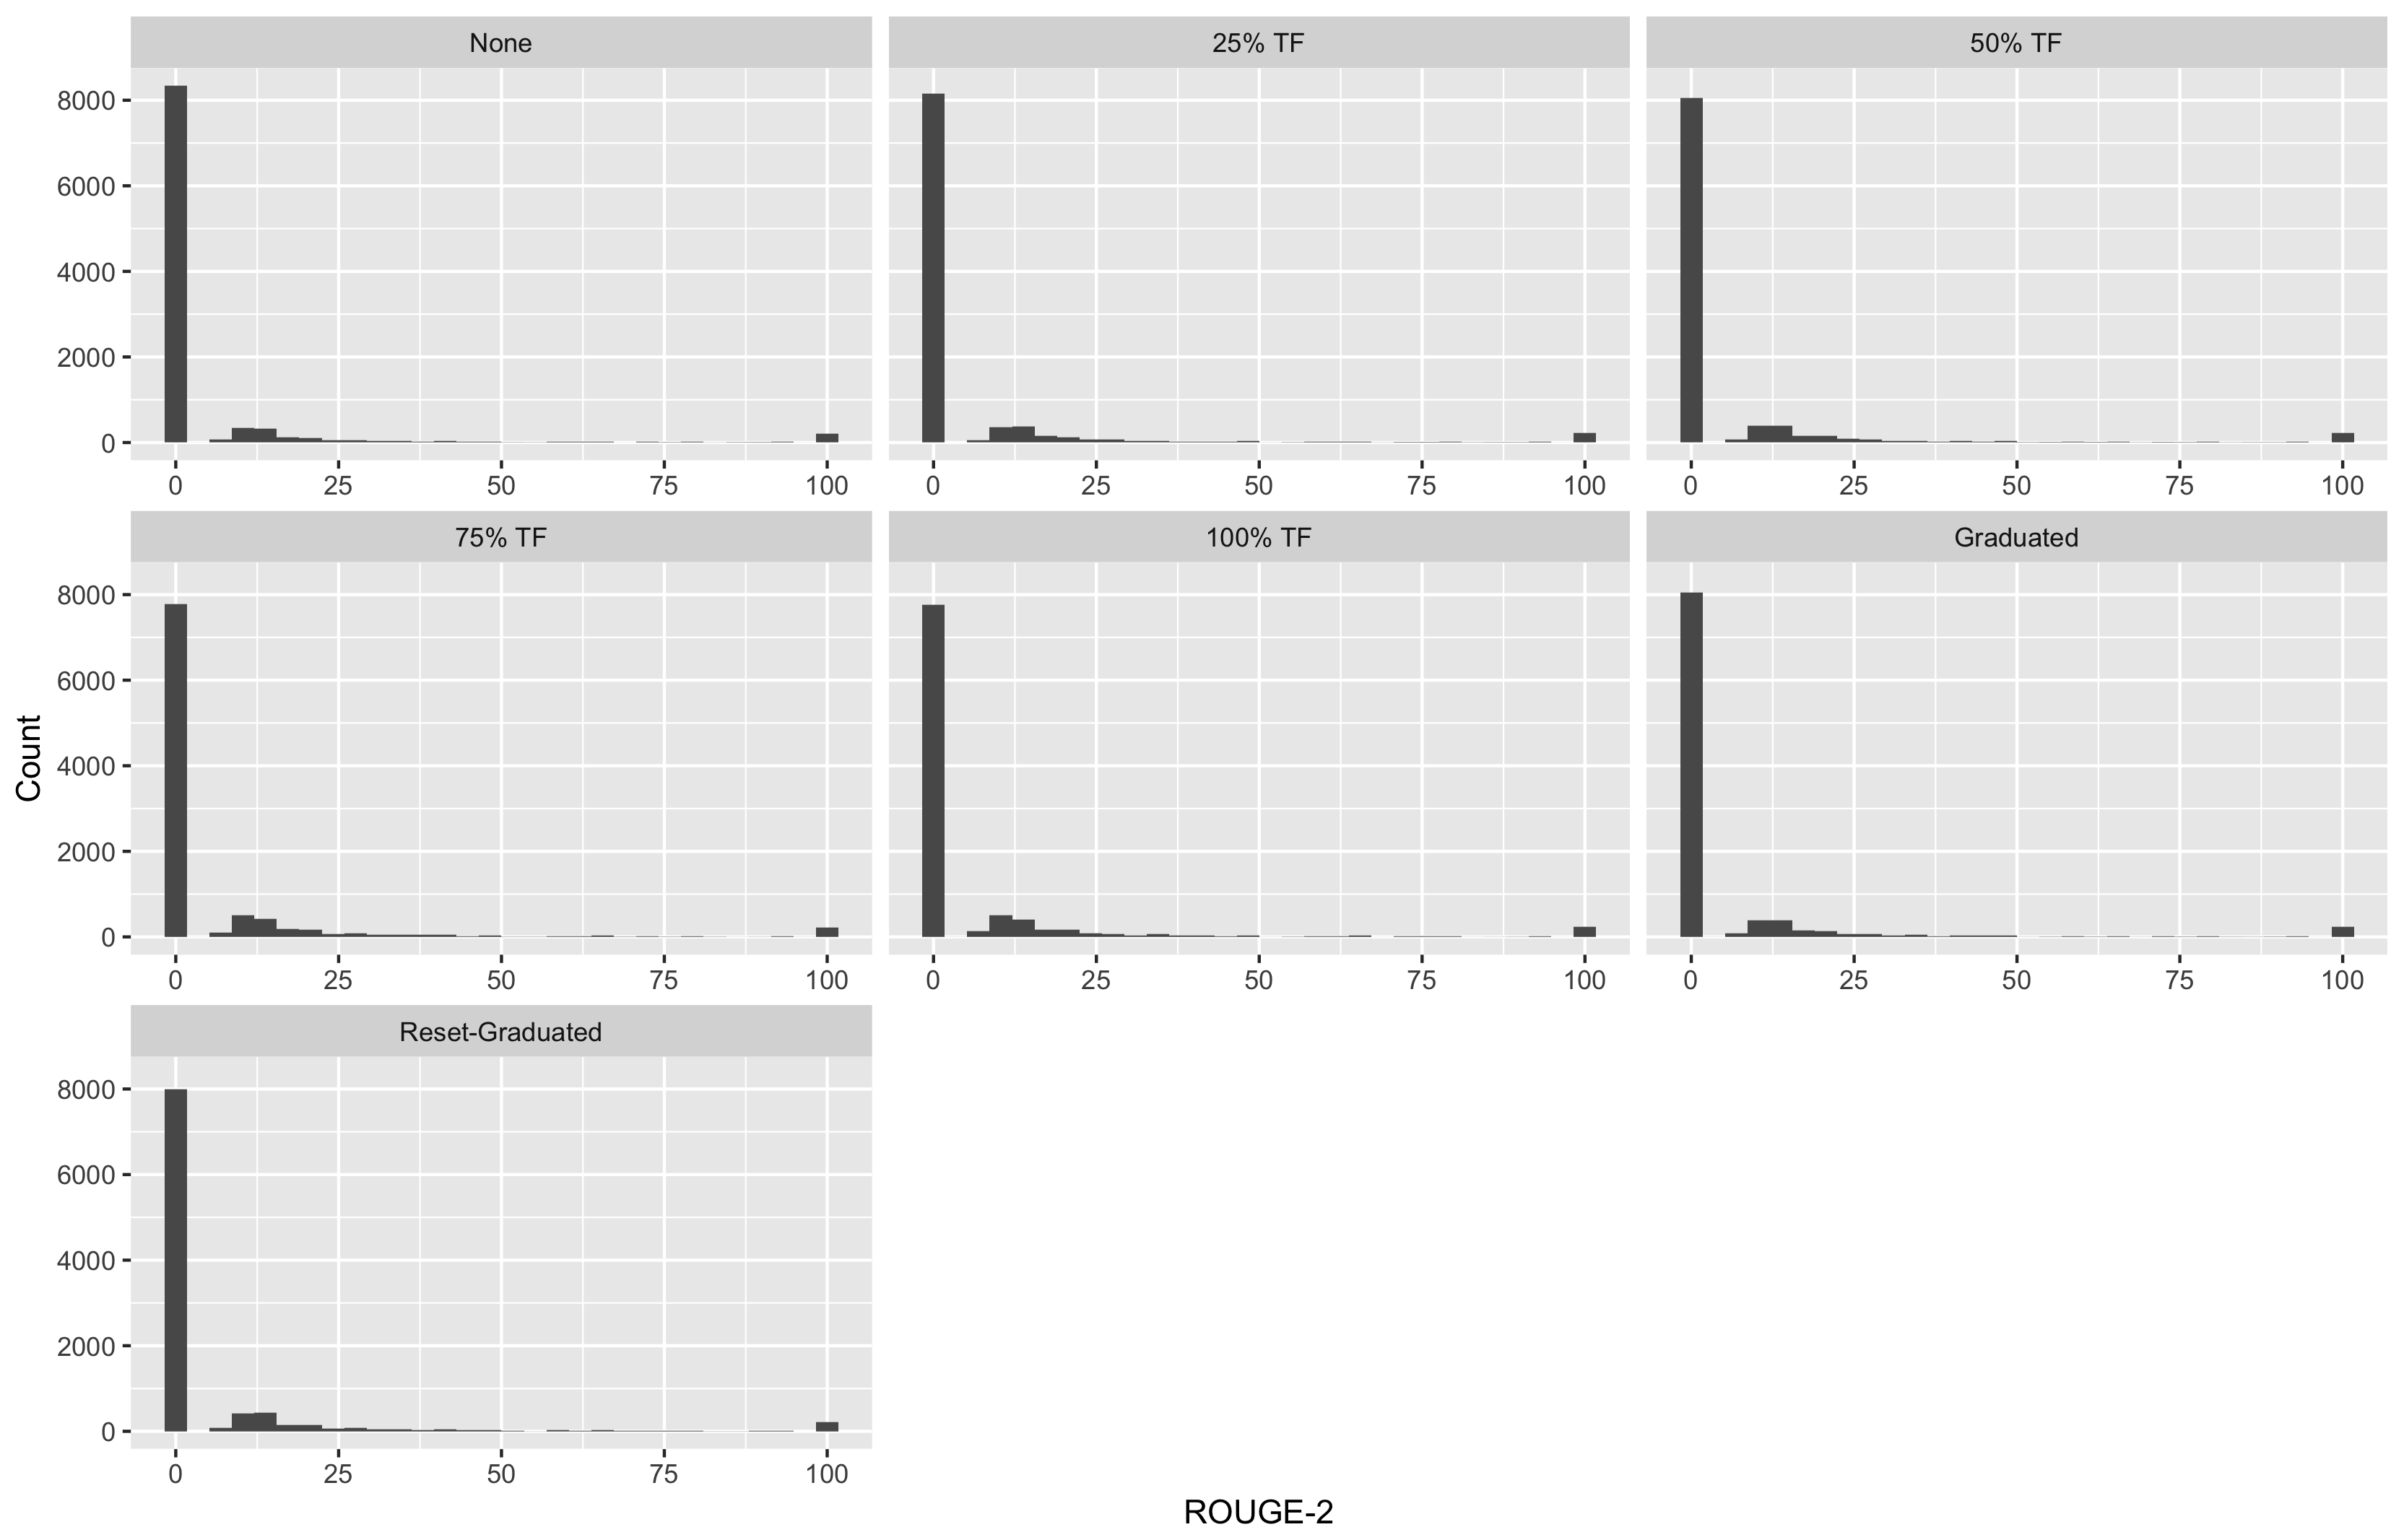
\includegraphics[width=0.8\textwidth]{../plots/test2/r2hists}
  \caption{Histograms of ROUGE-2 scores from all TF methods of Test 2}
  \label{fig:r2hists}
\end{figure}

Data non-normality can also be visualized via Q-Q Plots, as demonstrated for ROUGE-1 scores in Figure~\ref{fig:qqs}. A normal distribution would lie primarily near the regression line with dots randomly dispersed on either side~\cite{Ford2015}.

\begin{figure}[h]
  \centering
  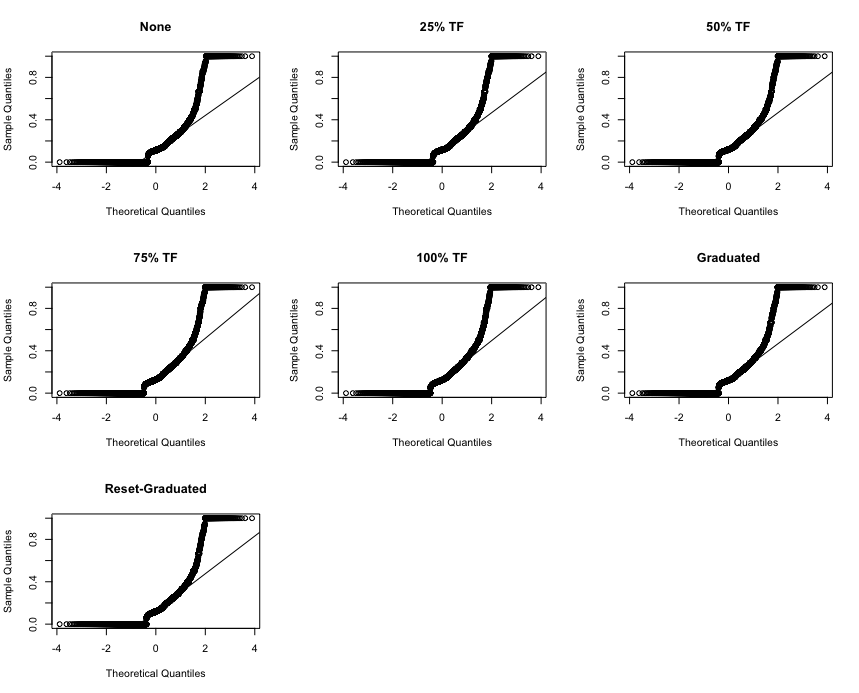
\includegraphics[width=0.8\textwidth]{../plots/test2/qqs}
  \caption{Q-Q Plots of ROUGE-1 scores for each TF Method of Test 2}
  \label{fig:qqs}
\end{figure}

Due to this skewedness, a Kruskal-Wallis test was used to compare the ROUGE results for each TF method across the three different tests. The results of the Kruskal-Wallis test can be viewed in Table~\ref{tab:kruskal}.

\begin{table}[h]
  \centering
  \begin{tabular}{| l | c | c |}
    \hline
    TF Method & ROUGE-1 & ROUGE-2\\
    \hline
    0\% & 0.481 & 0.262  \\
    25\% & 0.132 & 0.201  \\
    50\% & 0.162 & 0.307  \\
    75\% & 0.465 & 0.493  \\
    100\% & 0.632 & 0.577  \\
    Graduated & 0.175 & 0.770  \\
    Reset-Grad & 0.861 & 0.402  \\
    \hline
  \end{tabular}
  \caption{Kruskal-Wallis ROUGE-1 and ROUGE-2 p-values for various TF methods across three tests}
  \label{tab:kruskal}
\end{table}

Recall that values above 0.05 indicate a lack of statistical difference between the distributions of the data. Because all data fell within tolerance, we can safely assume no individual test benefitted from random chance. From here forward, analysis has only been conducted on the test 2. Having visualized the distribution of ROUGE scores and consolidated the analysis, we can now incorporate the appropriate metric for comparing TF methods: Wilcoxon averages and significance testing.

\subsubsection{Averages}\label{avg}
Tables~\ref{tab:avgROUGE1} and~\ref{tab:avgROUGE2} show the averages for ROUGE-1 and ROUGE-2, respectively. It bears repeating that, due to the necessary decrease in seq2seq architecture complexity, state-of-the-art results should not be expected. Rather, we are only hoping to compare various TF methods across the same datasets.

\begin{table}[h]
  \centering
  \begin{tabular}{| l | c | c |}
    \hline
    TF Method & Lower Bound & Upper Bound \\
    \hline
    0\% & 15.27  & 16.09 \\
    25\% & 16.04 & 16.86 \\
    50\% & 16.60 & 17.45 \\
    75\% & 17.76 & 18.59 \\
    100\% & 17.58 & 18.45 \\
    Graduated & 16.65 & 17.49 \\
    Reset-Grad & 16.52 & 17.36 \\
    \hline
  \end{tabular}
  \caption{ROUGE-1 bootstrapping averages for various TF methods}
  \label{tab:avgROUGE1}
\end{table}

\begin{table}[h]
  \centering
  \begin{tabular}{| l | c | c |}
    \hline
    TF Method & Lower Bound & Upper Bound \\
    \hline
    0\% & 4.997 & 5.688 \\
    25\% & 5.510 & 6.241 \\
    50\% & 5.692  & 6.403  \\
    75\% & 6.194  & 6.893  \\
    100\% & 6.223  & 6.964  \\
    Graduated & 5.692 & 6.421  \\
    Reset-Grad & 5.743 & 6.433  \\
    \hline
  \end{tabular}
  \caption{ROUGE-2 bootstrapping averages for various TF methods}
  \label{tab:avgROUGE2}
\end{table}

Perhaps surprisingly, these results appear to indicate that the highest levels of constantly held TF, 100\% and 75\%, resulted in the best possible ROUGE scores. This would appear to contradict the accepted wisdom that continual high levels of TF cause generative degradation. To validate these, though, we need to run paired Wilcoxon tests to test for significance.

\subsubsection{Paired Wilcoxon Tests}
We will run paired Wilcoxon tests on three different reference tests: all TF methods relative to no TF, all TF methods relative to 100\% TF, and graduated compared to reset-graduated. Recall from Section~\ref{stat} that the values reported are probabilities (p-values) that the differences in $\mu$ of the compared TF methods is 0. P-values $>$ 0.05 represent no statistically significant difference. We will first evaluate p-values with respect to no TF.

\begin{table}[h]
  \centering
  \begin{tabular}{| l | c | c |}
    \hline
    TF Method & ROUGE-1 & ROUGE-2 \\
    \hline
    25\% & 2.59E-3 & 9.77E-4  \\
    50\% & 2.46E-08 & 3.29E-07  \\
    75\% & 2.20E-16 & 2.20E-16  \\
    100\% & 2.20E-16 & 2.20E-16  \\
    Graduated & 1.43E-08 & 1.75E-7 \\
    Reset-Grad & 8.39E-08 & 6.57E-10  \\
    \hline
  \end{tabular}
  \caption{ROUGE paired Wilcoxon tests for various TF methods as compared to no teacher forcing}
  \label{tab:pairedNone}
\end{table}

It is immediately obvious that there are substantive differences between all TF methods relative to no TF, the least of which, unsurprisingly, being 25\% TF. Coupled with the fact that all TF methods had higher average confidence intervals, it is safe to assume that all TF methods under the parameters of the experiment score a higher ROUGE than not using TF. A simple ``greater-than'' Wilcoxon test confirms this to be true. Next we will evaluate all TF methods compared to 100\% TF, the industry standard at the moment.

\begin{table}[h]
  \centering
  \begin{tabular}{| l | c | c |}
    \hline
    TF Method & ROUGE-1 & ROUGE-2 \\
    \hline
    0\% & 2.20E-16 & 2.20E-16  \\
    25\% & 2.73E-10 & 1.15E-10  \\
    50\% & 1.81E-04 & 3.55E-06  \\
    75\% & 0.153 & 0.883  \\
    Graduated & 2.58E-04 & 5.78E-06  \\
    Reset-Grad & 8.14E-05 & 3.47E-4  \\
    \hline
  \end{tabular}
  \caption{ROUGE paired Wilcoxon tests for various TF methods as compared to 100\% teacher forcing}
  \label{tab:paired100}
\end{table}

Surprisingly, the differences in averages for 75\% and 100\% in Section~\ref{avg} seem to be substantiated by these paired Wilcoxon tests. We can see that 100\% teacher forcing is significantly different and of higher average confidence interval (See Sec.~\ref{avg}) than all TF methods besides 75\%. A ``greater-than'' Wilcoxon test confirms that these two TF methods have a statistically significantly higher mean than all other TF methods. Under the simplified conditions of this experiment, conventional wisdom is statistically incorrect. Because this project originally set out to research the effect of reset-graduated and graduated TF methods, we will analyze the statistical differences next, displayed in Figures~\ref{tab:pairedg}~and~\ref{tab:pairedrg}.

\begin{table}[h]
  \centering
  \begin{tabular}{| l | c | c | c | c |}
    \hline
    TF Method & ROUGE-1 & ROUGE-2 \\
    \hline
    0\% & 1.43E-08 & 1.75E-07  \\
    25\% & 7.79E-03 & 5.55E-2  \\
    50\% & 0.933 & 0.912  \\
    75\% & 3.72E-07 & 1.24E-05  \\
    100\% & 2.58E-04 & 5.78E-06  \\
    Reset-Grad & 0.778 & 0.343  \\
    \hline
  \end{tabular}
  \caption{ROUGE paired Wilcoxon tests for various TF methods as compared to graduated}
  \label{tab:pairedg}
\end{table}

\begin{table}[h]
  \centering
  \begin{tabular}{| l | c | c |}
    \hline
    TF Method & ROUGE-1 & ROUGE-2 \\
    \hline
    0\% & 8.38E-08  & 6.57E-10  \\
    25\% & 1.82E-2  & 4.23E-3  \\
    50\% & 0.842  & 0.292  \\
    75\% & 8.78E-08  & 6.31E-04  \\
    100\% & 8.14E-05  & 3.74E-04  \\
    Graduated & 0.778  & 0.343  \\
    \hline
  \end{tabular}
  \caption{ROUGE paired Wilcoxon tests for various TF methods as compared to reset-graduated}
  \label{tab:pairedrg}
\end{table}

As can be seen, graduated and reset-graduated TF methods have no statistically significant difference in generative performance. Perhaps unsurprisingly, both graduated and reset-graduated TF score similarly to 50\% constant TF, as these methods will, on average, have contributed TF approximately 50\% of the time. This is in contrast to the idea of presumed benefit from gradual tapering of TF, however.

Now that we have analyzed these various averages and their statistical differences, we will move on to loss over time.

\subsection{Loss over Time}\label{loss}
The original motivation behind TF was to speed up training. Consequently, we will evaluate the speed of convergence for all seven TF methods in all three tests conducted.

\begin{figure}[h]
  \centering
  Test 1 Losses\\
  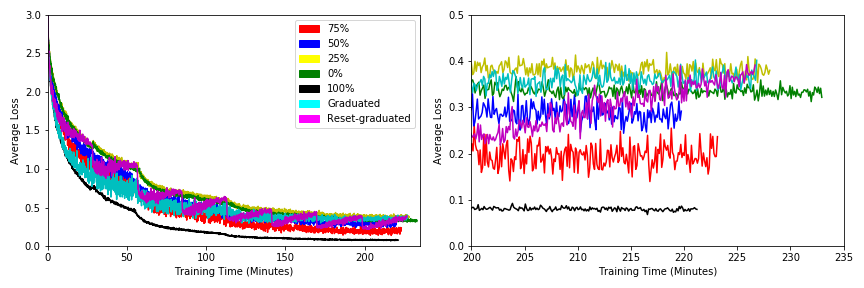
\includegraphics[width=0.8\textwidth]{../plots/test1comb}
  \caption{Average loss over time for every TF method for test 1}
  \label{fig:t1loss}
\end{figure}

\begin{figure}[h]
  \centering
  Test 2 Losses\\
  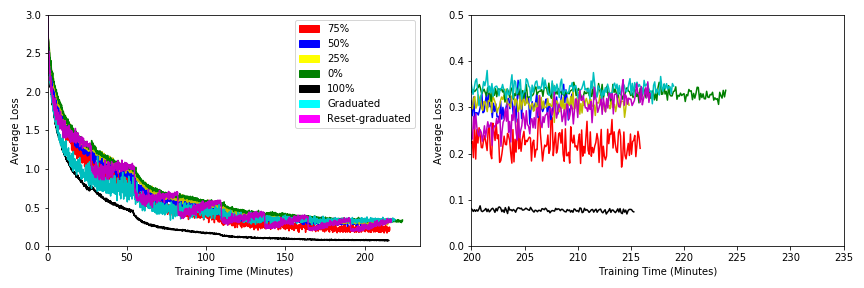
\includegraphics[width=0.8\textwidth]{../plots/test2comb}
  \caption{Average loss over time for every TF method for test 2}
  \label{fig:t2loss}
\end{figure}

\begin{figure}[h]
  \centering
  Test 3 Losses\\
  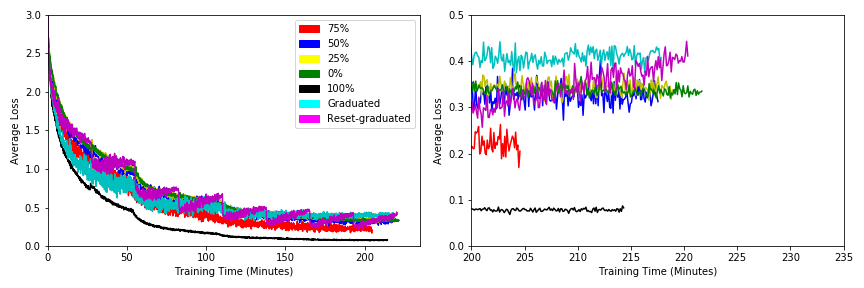
\includegraphics[width=0.8\textwidth]{../plots/test3comb}
  \caption{Average loss over time for every TF method for test 3}
  \label{fig:t3loss}
\end{figure}

There is a definite pattern amongst these three plots. 100\% TF converges noticably faster than all other TF tests. Additionally, 100\% TF had the lowest loss, unsurprising given the ROUGE findings. 75\% TF is consistently the second lowest for coverged loss. The rest all fall within the same general vacinity of one another. One interesting observation is how the Kruskal-Wallis scores showed no statistical difference between any of the ROUGE tests, yet many of the models from these techniques fluctuate by as much as 0.05. This would indicate that ROUGE outcomes are not particularly susceptible to such fluctuations at this loss level.

A second interesting observation is that converged loss proximity does not align with statistically significant over-performance on the ROUGE metric. According to the analysis on test 2 in Section~\ref{avg}, graduated, reset-graduated, 50\% and even 25\% all statistically outperformed 0\% TF, yet all final loss values are roughly the same. Indeed,  pulling the last recorded average loss for the functions results in the following losses:

\begin{itemize}
\item Graduated: 0.346
\item Reset-graduated: 0.329
\item 50\%: 0.327
\item 25\%: 0.305
\item 0\%: 0.337
\end{itemize}

This discrepancy between significant out-performance on ROUGE and comparative final loss values raises questions of whether ROUGE is a reliable metric, or whether the traditional cost function for these models needs could be better suited to specifically maximize ROUGE scores. However, given the lack of sophistication involved in ROUGE, I'm willing to bet the former. These observations raise some interesting new questions for future research.